\documentclass[aspectratio=169, 10pt]{beamer}

% Theme reusado de la versión anterior (assets en ../)
\usetheme{focus}

% Paleta SupaClock
\definecolor{main}{RGB}{57, 110, 184}
\definecolor{background}{RGB}{255, 255, 255}
\definecolor{accent}{RGB}{63, 185, 80}      % verde algoritmo
\definecolor{warn}{RGB}{218, 54, 51}        % rojo problema

\setbeamercolor{alerted text}{fg=red!80!black}

\usepackage[spanish]{babel}
\usepackage[utf8]{inputenc}
\usepackage{graphicx}
\usepackage{booktabs}
\usepackage{tikz}
\usepackage{pgfplots}
\pgfplotsset{compat=1.18}
\usetikzlibrary{shapes.geometric, arrows.meta, positioning, fit, backgrounds, calc, babel, patterns}

\setbeamerfont{itemize/enumerate body}{size=\small}
\setbeamerfont{itemize/enumerate subbody}{size=\footnotesize}

% Recursos compartidos con la versión anterior están en ../
\graphicspath{{../}{../../}{../../../tools/}}

\title{Wearable ``SupaClock''}
\subtitle{Reporte de Avance 25\% \textbar{} Validaci\'on de Subsistemas}
\date{\today}
\author{Grupo 10}
\institute{Ingenier\'ia El\'ectrica}
\titlegraphic{\hfill
\includegraphics[height=1.8cm]{logo.pdf}}

\begin{document}

% ═══════════════════════════════════════════════════════════════════
\maketitle
% ═══════════════════════════════════════════════════════════════════

% ─── Slide 2 — Visión + agenda ───
\begin{frame}{Visi\'on del producto y agenda}
    \begin{columns}[T]
        \column{0.55\textwidth}
        \textbf{SupaClock}: wearable de monitoreo biom\'etrico continuo con enfoque cl\'inico ``Cero distracciones'', orientado a personal m\'edico.
        \vspace{0.2cm}
        \begin{itemize}
            \item ECG, frecuencia cardiaca, SpO\textsubscript{2}, temperatura corporal, podometr\'ia
            \item Telemetr\'ia BLE en vivo a equipo m\'edico
            \item Procesamiento on-device + clasificador de actividad por ML
        \end{itemize}
        \column{0.45\textwidth}
        \fbox{\parbox{0.95\linewidth}{\centering \scriptsize\textit{[Placeholder: hero\_render.png — render del producto]}\\\vspace{0.3cm}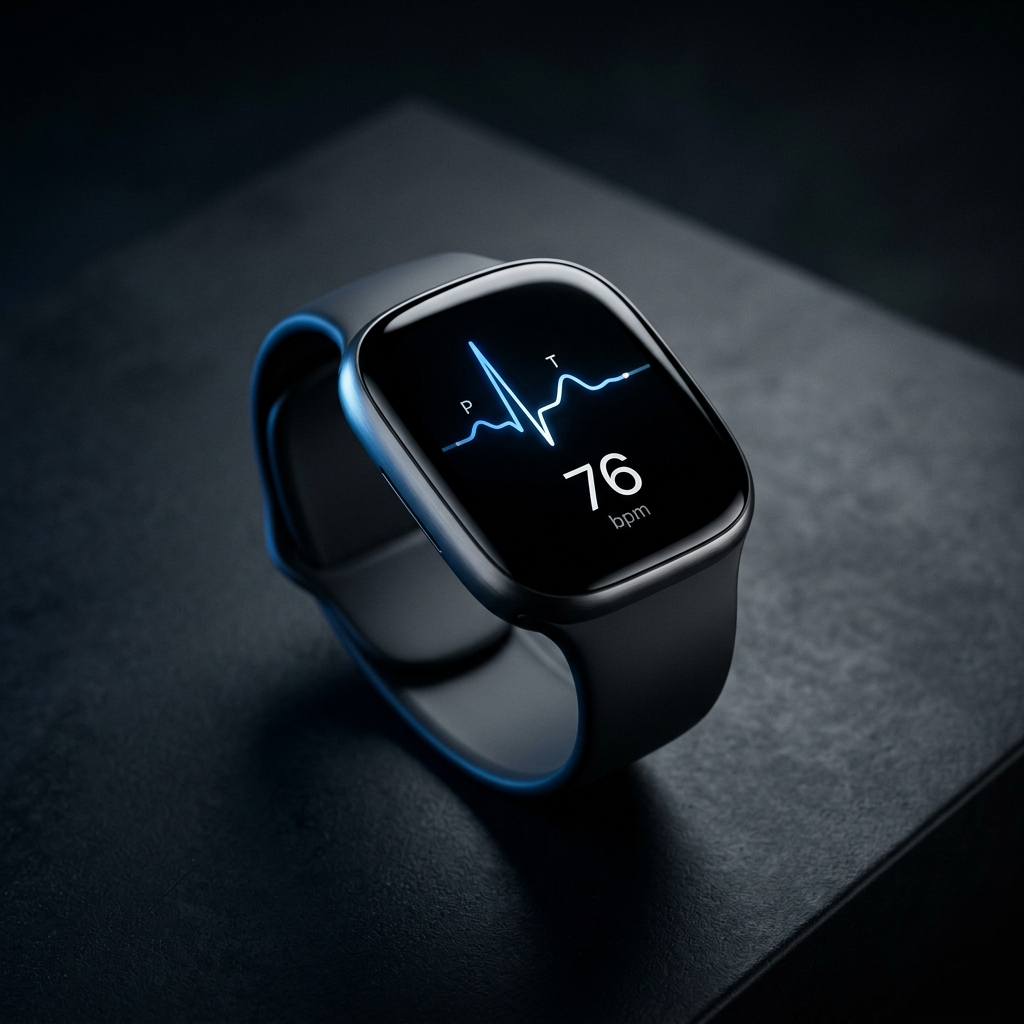
\includegraphics[width=\linewidth, keepaspectratio]{hero_render.png}}}
    \end{columns}
    \vspace{0.3cm}
    \footnotesize
    \textbf{Agenda} (10 min): Hardware $\rightarrow$ Firmware y algoritmos $\rightarrow$ Comunicaci\'on, m\'etricas y futuro.
\end{frame}

% ═══════════════════════════════════════════════════════════════════
\section{Hardware e Integraci\'on}
% ═══════════════════════════════════════════════════════════════════

% ─── Slide 3 — Ecosistema HW ───
\begin{frame}{Ecosistema de Hardware: 6 sensores integrados}
    \begin{columns}[T]
        \column{0.42\textwidth}
        \scriptsize
        \begin{tabular}{l l}
            \toprule
            \textbf{Componente} & \textbf{Bus} \\
            \midrule
            BMI160 (IMU 6-DOF)        & I\textsuperscript{2}C 0x68 \\
            MAX30102 (PPG/HR/SpO\textsubscript{2}) & I\textsuperscript{2}C 0x57 \\
            MAX30205 (Temp corporal)  & I\textsuperscript{2}C 0x48 \\
            MAX17048 (Fuel gauge)     & I\textsuperscript{2}C 0x36 \\
            AD8232 (ECG)              & ADC1 + DMA \\
            ST7789 (Display 240\(\times\)280) & SPI 80\,MHz \\
            \bottomrule
        \end{tabular}
        \vspace{0.3cm}
        \begin{itemize}
            \item Bus I\textsuperscript{2}C compartido a \textbf{400 kHz}
            \item Mutex global protege accesos concurrentes
            \item ECG por DMA continuo (no compite por I\textsuperscript{2}C)
        \end{itemize}
        \column{0.58\textwidth}
        \fbox{\parbox{0.95\linewidth}{\centering \scriptsize\textit{[Diagrama ecosistema reutilizado de Entrega1]}\\\vspace{0.2cm}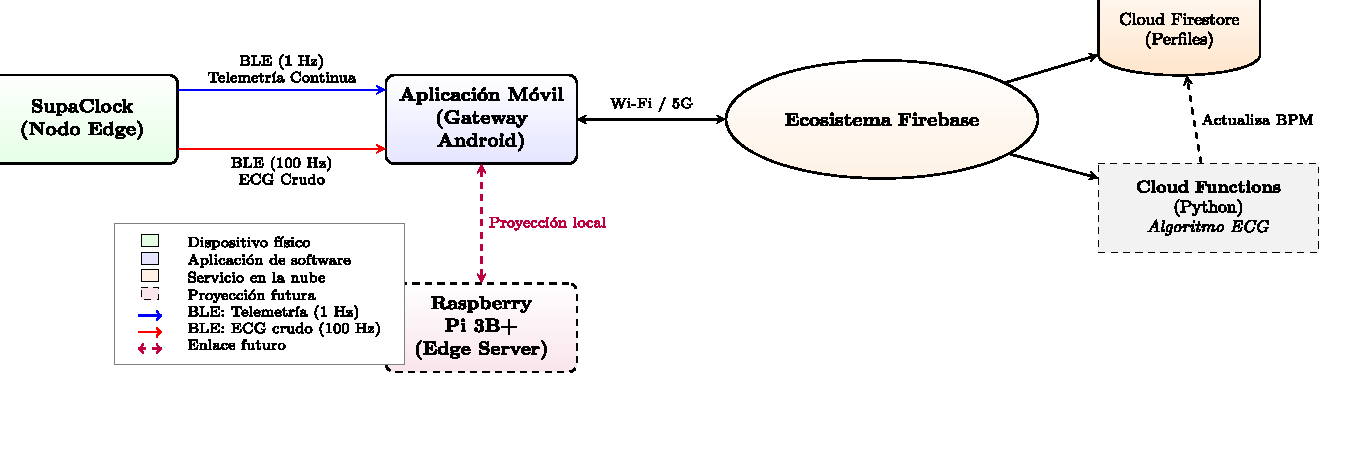
\includegraphics[width=0.9\linewidth, keepaspectratio]{Entrega1/diag_ecosistema.pdf}}}
    \end{columns}
\end{frame}

% ─── Slide 4 — Subsistema energía + LDO + PCB ───
\begin{frame}{Subsistema de Energ\'ia y PCB Prototipo}
    \begin{columns}[T]
        \column{0.55\textwidth}
        \begin{itemize}
            \item \textbf{BMS}: TP4056 (carga LiPo) + DW01A (protecci\'on sobre/sub-tensi\'on)
            \item \textbf{Fuel gauge}: MAX17048 reporta voltaje y SoC por I\textsuperscript{2}C
            \item \textbf{Regulador (C3 SuperMini)}: LDO ME6211 \alert{\textbf{insuficiente}} para picos de radio + sensores
        \end{itemize}
        \vspace{0.2cm}
        \begin{alertblock}{Problema detectado}
            \scriptsize Reset por brownout al activar BLE concurrente con bursts del display. Pico medido $\sim$\textbf{110\,mA} en bater\'ia (probablemente subestimado por la respuesta del amper\'imetro).
        \end{alertblock}
        \column{0.45\textwidth}
        \fbox{\parbox{0.95\linewidth}{\centering \scriptsize\textit{[Placeholder: foto de PCB no-SMD prototipo]}\\\vspace{1cm}foto pendiente\\\vspace{1cm}}}
        \vspace{0.2cm}
        \scriptsize \textit{La PCB through-hole con C3 SuperMini est\'a en montaje; en paralelo se encarg\'o la siguiente revisi\'on con ESP32-S3 (slide 12).}
    \end{columns}
\end{frame}

% ═══════════════════════════════════════════════════════════════════
\section{Firmware y Algoritmos}
% ═══════════════════════════════════════════════════════════════════

% ─── Slide 5 — Arquitectura SW + tasks + modos ───
\begin{frame}{Arquitectura de Software: 6 tareas FreeRTOS + Modos de Energ\'ia}
    \begin{columns}[T]
        \column{0.46\textwidth}
        \scriptsize
        \begin{tabular}{l c c}
            \toprule
            \textbf{Tarea} & \textbf{Prio} & \textbf{Cadencia} \\
            \midrule
            \texttt{ecg\_task}     & 7 & DMA continuo \\
            \texttt{imu\_task}     & 6 & 50/25/12.5\,Hz\textsuperscript{*}\\
            \texttt{hrm\_task}     & 5 & SM (modo) \\
            \texttt{gui\_task}     & 5 & 30\,FPS \\
            \texttt{ble\_tx\_task} & 4 & flush peri\'odico \\
            \texttt{system\_task}  & 3 & 30\,s / 5\,min \\
            \bottomrule
        \end{tabular}
        \vspace{0.15cm}
        \scriptsize\textit{\textsuperscript{*}seg\'un modo de energ\'ia activo.}
        \vspace{0.3cm}
        \textbf{Sincronizaci\'on}: \texttt{xSensorDataMutex} + mutex I\textsuperscript{2}C global.

        \column{0.54\textwidth}
        \scriptsize
        \begin{tabular}{l c c c}
            \toprule
             & \textbf{SPORT} & \textbf{NORMAL} & \textbf{SAVER} \\
            \midrule
            HR (MAX30102)    & continuo & cada 10\,min & cada 30\,min \\
            SpO\textsubscript{2}      & cada 5\,min & cada 30\,min & manual \\
            IMU              & 50\,Hz & 25\,Hz & 12.5\,Hz \\
            Temp             & 30\,s & 5\,min & 15\,min \\
            Bater\'ia        & 30\,s & 30\,s & 30\,s \\
            BLE flush        & 1\,s & 10\,s & 60\,s \\
            Auto-off         & 30\,s & 15\,s & 8\,s \\
            \bottomrule
        \end{tabular}
        \vspace{0.2cm}
        \begin{itemize}
            \item Selecci\'on manual desde men\'u; persistencia en NVS
            \item En NORMAL/SAVER, MAX30102 entra a SHDN ($\sim$0.7\,$\mu$A)
        \end{itemize}
    \end{columns}
\end{frame}

% ─── Slide 6 — Pipeline HR/SpO2 ───
\begin{frame}{Pipeline HR/SpO\textsubscript{2}: comparativa con Galaxy Watch}
    \begin{columns}[T]
        \column{0.50\textwidth}
        \footnotesize
        \textbf{Captura PPG}: Red + IR a 25\,Hz efectivos (100\,sps, \texttt{SMP\_AVE=4}).
        \vspace{0.15cm}
        \textbf{Pipeline}:
        \begin{enumerate}\itemsep0pt
            \item Tracker DC (EMA \(\alpha\)=0.05)
            \item \textbf{Bandpass IIR Butterworth 0.5--4\,Hz} (cascada HPF + LPF)
            \item Detector de picos con umbral adaptativo
            \item \textbf{Mediana de 8 RR} con rechazo de outliers ($\Delta$RR$>$25\%)
            \item SpO\textsubscript{2}: \textbf{mediana m\'ovil de 10 valores R}
            \item \textbf{Motion gating}: jerk del IMU invalida muestras
        \end{enumerate}
        \vspace{0.15cm}
        \textbf{Modo SPOT dedicado} (estilo Galaxy Watch): 12--30\,s con \textit{early-exit} cuando $\sigma$/$\mu$ de RR $<$ 8\% y $\sigma$/$\mu$ de R $<$ 5\%.
        \column{0.50\textwidth}
        \fbox{\parbox{0.95\linewidth}{\centering \scriptsize\textit{[Placeholder: comparativa antes/despu\'es del bandpass IIR -- generar con \texttt{tools/supaclock\_raw\_ppg.py} y env:test\_spo2]}\\\vspace{2.5cm}raw\_ppg\_*.png pendiente\\\vspace{2.5cm}}}
    \end{columns}
\end{frame}

% ─── Slide 7 — ECG Pan-Tompkins ───
\begin{frame}{ECG: Adquisici\'on y Pan-Tompkins}
    \begin{columns}[T]
        \column{0.48\textwidth}
        \footnotesize
        \textbf{Adquisici\'on}:
        \begin{itemize}\itemsep0pt
            \item AD8232 + ADC continuo con DMA a \textbf{20\,kHz}
            \item Diezmado por factor \(\times\)40 $\rightarrow$ stream BLE a \textbf{500\,Hz}
            \item Caracter\'istica BLE 0xFF03 dedicada
        \end{itemize}
        \vspace{0.15cm}
        \textbf{Pan-Tompkins} (offline en host):
        \begin{enumerate}\itemsep0pt
            \item Bandpass 5--15\,Hz (banda QRS)
            \item Derivada (resalta pendientes)
            \item Cuadratura
            \item Integraci\'on en ventana m\'ovil
            \item Detecci\'on de picos R con umbral adaptativo
        \end{enumerate}
        \column{0.52\textwidth}
        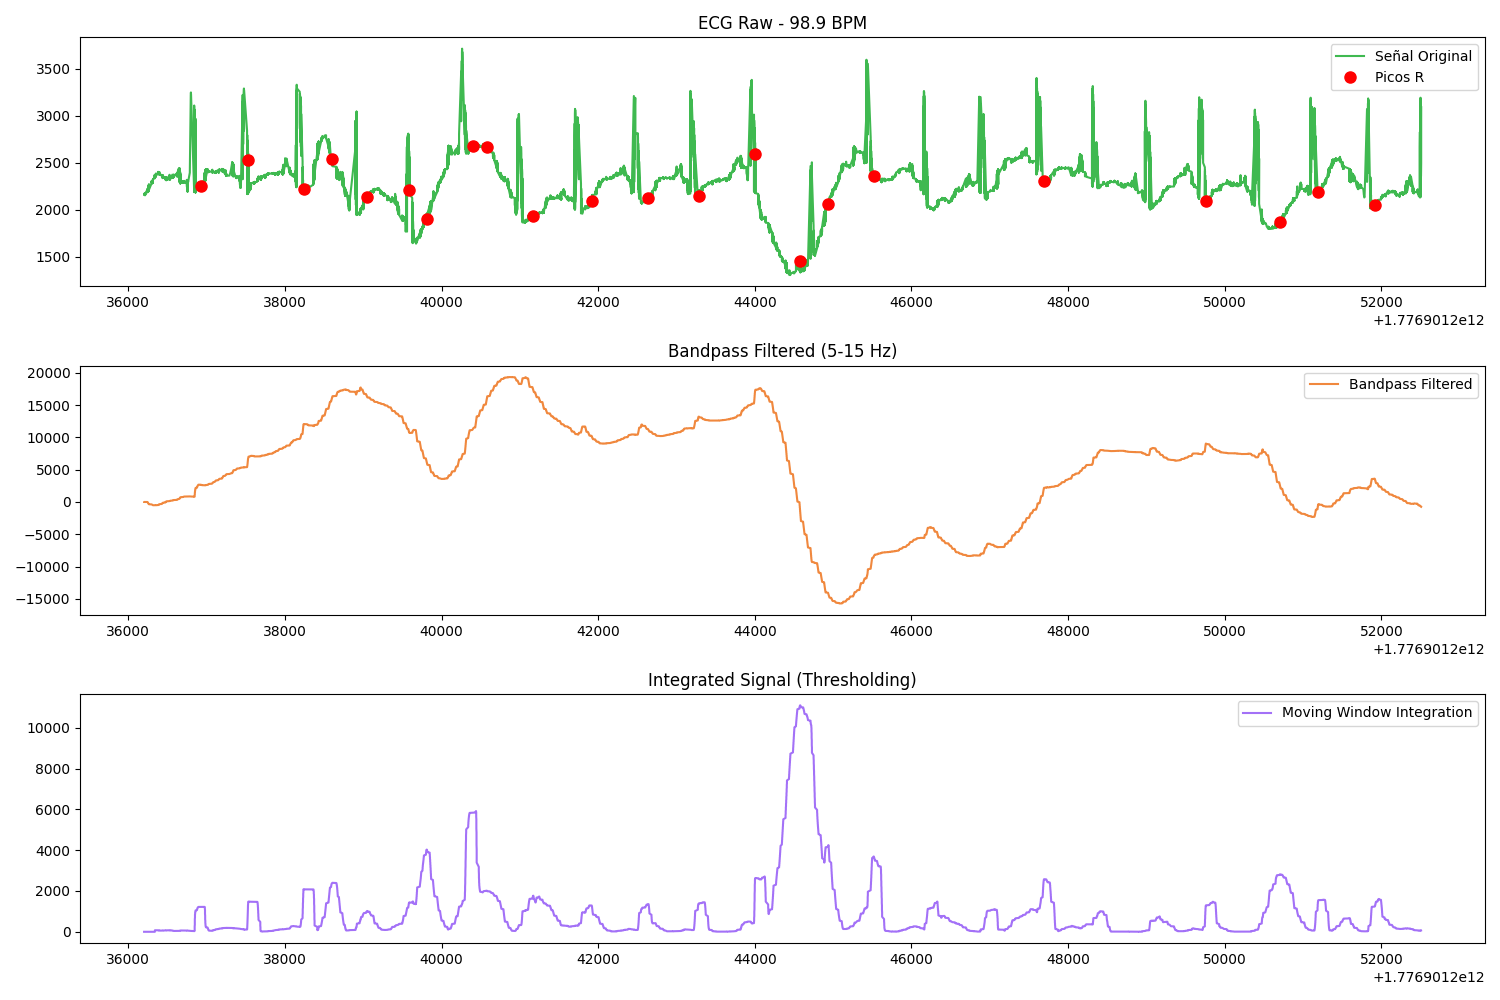
\includegraphics[width=\linewidth, keepaspectratio]{pan_tompkins_results.png}
        \vspace{-0.2cm}
        \scriptsize\textit{Resultado sobre captura del AD8232 (CSV).}
    \end{columns}
\end{frame}

% ─── Slide 8 — Podómetro tiempo vs frecuencia ───
\begin{frame}{Pod\'ometro: del dominio del tiempo al de la frecuencia}
    \begin{columns}[T]
        \column{0.42\textwidth}
        \footnotesize
        \textbf{Implementaci\'on actual} (dominio tiempo):
        \begin{enumerate}\itemsep0pt
            \item Magnitud 3D del acelerador
            \item Filtro media m\'ovil (10 muestras)
            \item Detector de picos con umbral adaptativo (re-evaluaci\'on cada 5\,s)
        \end{enumerate}
        \vspace{0.15cm}
        \alert{\textbf{Limitaci\'on detectada}}: agitar la mano emula picos $\rightarrow$ falsos positivos.
        \vspace{0.2cm}
        \textbf{Soluci\'on planificada} (dominio frecuencia):
        \begin{itemize}\itemsep0pt
            \item FFT sobre ventana de 3\,s
            \item Validar cadencia r\'itmica (1--3\,Hz)
            \item Requiere DSP vectorial $\rightarrow$ ESP32-S3
        \end{itemize}
        \column{0.58\textwidth}
        
\includegraphics[width=\linewidth, keepaspectratio]{simulation_results.png}
        \vspace{-0.2cm}
        \scriptsize\textit{Resultado del algoritmo en tiempo (CSV con 56 pasos reales).}
    \end{columns}
\end{frame}

% ─── Slide 9 — Validación tests modulares ───
\begin{frame}{Validaci\'on por subsistemas: 9 environments PlatformIO}
    \footnotesize
    Cada sensor / m\'odulo cuenta con su propio firmware de prueba aislado, m\'as un firmware integrador (\texttt{test\_general}).
    \vspace{0.2cm}
    \begin{columns}[T]
        \column{0.45\textwidth}
        \begin{tabular}{l l}
            \toprule
            \textbf{Env} & \textbf{Subsistema} \\
            \midrule
            \texttt{test\_temp}        & MAX30205 \\
            \texttt{test\_imu}         & BMI160 + step\_algo \\
            \texttt{test\_spo2}        & MAX30102 raw + BLE \\
            \texttt{test\_ecg}         & AD8232 ADC/DMA \\
            \texttt{test\_display}     & ST7789 + LVGL \\
            \texttt{test\_ble}         & NimBLE GATT \\
            \texttt{test\_fuel\_gauge} & MAX17048 \\
            \texttt{test\_gui}         & Navegaci\'on GUI \\
            \texttt{test\_general}     & \textbf{Integrador} \\
            \bottomrule
        \end{tabular}
        \column{0.55\textwidth}
        \begin{itemize}\itemsep0pt
            \item Cada \texttt{test\_*} se compila y flashea independiente
            \item Permite aislar fallas de driver vs integraci\'on
            \item \texttt{test\_general} ejecuta los 6 sensores + GUI + BLE simult\'aneamente $\rightarrow$ valida concurrencia, mutex, modos de energ\'ia
            \item Demo en vivo se hace con \texttt{test\_general}
        \end{itemize}
    \end{columns}
\end{frame}

% ═══════════════════════════════════════════════════════════════════
\section{Comunicaci\'on, M\'etricas y Futuro}
% ═══════════════════════════════════════════════════════════════════

% ─── Slide 10 — BLE + monitor + base ML ───
\begin{frame}{Stack BLE y herramienta de validaci\'on}
    \begin{columns}[T]
        \column{0.50\textwidth}
        \footnotesize
        \textbf{4 caracter\'isticas BLE} (GATT custom 0xFF00):
        \begin{itemize}\itemsep0pt
            \item \texttt{0xFF01} IMU 6-DOF (12 B/notify, 50\,Hz)
            \item \texttt{0xFF02} Telemetr\'ia agregada \textbf{TLV} (HR, SpO\textsubscript{2}, temp, bat, eventos modo)
            \item \texttt{0xFF03} ECG streaming (chunks 500\,Hz)
            \item \texttt{0xFF04} Comandos RX (host $\rightarrow$ reloj)
        \end{itemize}
        \vspace{0.1cm}
        El protocolo TLV permite agrupar muestras heterog\'eneas con timestamp y reduce overhead BLE en SAVER (1 paquete/min vs 60).
        \column{0.50\textwidth}
        \fbox{\parbox{0.95\linewidth}{\centering \scriptsize\textit{[Placeholder: screenshot supaclock\_monitor.py]}\\\vspace{0.5cm}herramienta PyQt6 +\\bleak + pyqtgraph + opengl\\\vspace{0.5cm}}}
        \vspace{0.15cm}
        \scriptsize
        \textbf{supaclock\_monitor.py} muestra IMU/ECG/biom\'etricos en vivo y graba CSV.\\
        \textbf{$\rightarrow$ Base de datos para entrenar el clasificador CNN 1D.}
    \end{columns}
\end{frame}

% ─── Slide 11 — Métricas reales ───
\begin{frame}{M\'etricas reales: CPU, RAM y Pila por tarea}
    \begin{columns}[T]
        \column{0.50\textwidth}
        \footnotesize
        \textbf{CPU (\texttt{vTaskGetRunTimeStats})}
        \vspace{-0.05cm}
        \begin{tikzpicture}
        \begin{axis}[
            xbar stacked,
            width=\linewidth, height=3.6cm,
            bar width=14pt,
            xmin=0, xmax=100,
            ytick=\empty, axis y line=none,
            xlabel={\scriptsize \% CPU},
            xlabel style={font=\scriptsize},
            tick label style={font=\scriptsize},
            legend style={
                at={(0.5,-0.30)}, anchor=north,
                font=\tiny,
                legend columns=4,
                draw=none,
                /tikz/every even column/.append style={column sep=0.2cm}
            },
            nodes near coords align={center}
        ]
        \addplot+[fill=gray!50, draw=gray!70] coordinates {(49,0)};
        \addplot+[fill=blue!50, draw=blue!70] coordinates {(47,0)};
        \addplot+[fill=red!60, draw=red!70]   coordinates {(1,0)};
        \addplot+[fill=green!60,draw=green!70] coordinates {(3,0)};
        \legend{IDLE 49\%, gui 47\%, imu 1\%, otros $<$1\%}
        \end{axis}
        \end{tikzpicture}

        \vspace{0.15cm}
        \scriptsize \textit{IDLE 49\,\%}: holgura ajustada en C3 single-core 160\,MHz.

        \column{0.50\textwidth}
        \footnotesize
        \textbf{Memoria}
        \scriptsize
        \begin{tabular}{l r}
            \toprule
            Heap libre actual    & 99\,104 B \\
            Heap m\'inimo hist\'orico & 93\,972 B \\
            Margen sobre 320\,KB SRAM & $\sim$30\,\% \\
            \bottomrule
        \end{tabular}
        \vspace{0.15cm}

        \textbf{Pila por tarea (HWM, libre)}\\[-0.15cm]
        \scriptsize
        \begin{tabular}{l r r}
            \toprule
            Tarea & Stack & Libre HWM \\
            \midrule
            ecg\_task     & 4096 & 3416 B \\
            system\_task  & 4096 & 3528 B \\
            imu\_task     & 4096 & 2144 B \\
            gui\_task     & 4096 & 2036 B \\
            hrm\_task     & 4096 & 1872 B \\
            ble\_tx\_task & \textbf{4096}\textsuperscript{\dag} & 960 B \\
            \bottomrule
        \end{tabular}
        \vspace{0.05cm}
        \scriptsize\textsuperscript{\dag}corregido tras detectar margen de 960 B en 3072 inicial.
    \end{columns}
\end{frame}

% ─── Slide 12 — Consumo y migración S3 ───
\begin{frame}{Consumo medido y migraci\'on a ESP32-S3}
    \begin{columns}[T]
        \column{0.50\textwidth}
        \footnotesize
        \textbf{Consumo en bater\'ia} (amper\'imetro en serie)
        \scriptsize
        \begin{tabular}{l r}
            \toprule
            Reposo, display off, BLE conectado & XX\,mA \\
            \textbf{SPORT} (todo activo) -- pico & \textbf{$\sim$110\,mA} \\
            \textbf{NORMAL} promedio              & XX\,mA \\
            \textbf{SAVER} promedio               & XX\,mA \\
            \bottomrule
        \end{tabular}
        \vspace{0.15cm}

        \footnotesize
        \begin{itemize}\itemsep0pt
            \item LDO ME6211 del C3 SuperMini limitado a $\sim$300\,mA continuos
            \item Picos transitorios de BLE+display+sensores activan brownout intermitente
        \end{itemize}
        \column{0.50\textwidth}
        \footnotesize
        \textbf{Soluci\'on: Seeed XIAO ESP32-S3} (encargada)
        \begin{itemize}\itemsep0pt
            \item \textbf{Buck SGM6029} integrado, 800\,mA $\rightarrow$ resuelve brownout
            \item Dual-core 240\,MHz + SIMD vectorial
            \item ESP-NN: inferencia CNN 1D 5--20\,ms vs 50--200\,ms en C3
            \item M\'as tiempo en \textit{light sleep} $\rightarrow$ menor consumo promedio
            \item BMS y monitor de carga en placa
        \end{itemize}
        \vspace{0.1cm}
        \scriptsize
        \textit{Migraci\'on motivada por \textbf{datos}: el 49\,\% de IDLE deja poco margen para la CNN 1D del clasificador.}
    \end{columns}
\end{frame}

% ─── Slide 13 — CNN 1D + próximos pasos ───
\begin{frame}{Pr\'oximos pasos y modelo de Machine Learning}
    \begin{columns}[T]
        \column{0.55\textwidth}
        \footnotesize
        \textbf{Clasificador de actividad — CNN 1D}
        \begin{itemize}\itemsep0pt
            \item \textbf{Entrada}: ventana 3\,s del IMU \(\rightarrow\) 6 canales \(\times\) 150 muestras
            \item \textbf{Arquitectura}: 2--3 capas Conv1D + GAP + Dense
            \item \textbf{Salida}: 4--5 clases (reposo / caminar / correr / agitar mano / dormir)
            \item Entrenamiento offline con CSV recolectados v\'ia \texttt{supaclock\_monitor.py}
            \item Despliegue en S3 v\'ia ESP-NN cuantizada int8
        \end{itemize}
        \column{0.45\textwidth}
        \footnotesize
        \textbf{Hito 50\,\%}
        \begin{enumerate}\itemsep0pt
            \item Validaci\'on de la S3 con todos los drivers actuales
            \item Migraci\'on del pod\'ometro a FFT (ESP-DSP)
            \item Recolecci\'on dataset de actividades reales
            \item Entrenamiento + cuantizaci\'on CNN 1D
            \item PCB SMD con S3 + sensores integrados
        \end{enumerate}
    \end{columns}
\end{frame}

% ═══════════════════════════════════════════════════════════════════
\begin{frame}[plain]
    \centering
    \vspace{1.5cm}
    {\Huge \color{main} \textbf{Demostraci\'on en vivo}}\\[0.6cm]
    {\Large 5\,min}\\[0.4cm]
    \footnotesize
    Navegaci\'on UI \textbar{} HR continuo \textbar{} SPOT dedicado \textbar{} cambio de modo \textbar{} ECG streaming\\
    Telemetr\'ia BLE en \texttt{supaclock\_monitor.py}
\end{frame}

\end{document}
